\documentclass[10pt,sans,english,compress,xcolor=dvipsnames]{beamer}
\author[Lily ]{ Dr Lily Asquith (Lily, she/her)}

\usetheme{Szeged}
%\defbeamertemplateparent{enumerate items}{enumerate item,enumerate subitem,enumerate subsubitem,enumerate mini template}
\definecolor{titcol}{RGB}{16,78,100} 
\setbeamercolor{frametitle}{fg=titcol,bg=White}
\useoutertheme{miniframes} 
\useinnertheme{rectangles}

\usepackage{pifont}
\newcommand{\tick}{\textcolor{grn}{\ding{52} } }
\newcommand{\nope}{\textcolor{red}{\ding{54} } }


\usepackage{soul}
\usepackage{cancel}

\usepackage[most]{tcolorbox}
\definecolor{LilyBlack}{rgb}{0.05,0.1,0.3} % UBC Blue (primary)
\usecolortheme[named=LilyBlack]{structure}

\usepackage{booktabs}
\usepackage{tabularx}
%\usepackage{tikz}
%\def\checkmark{\tikz\fill[scale=0.4](0,.35) -- (.25,0) -- (1,.7) -- (.25,.15) -- cycle;}

\usepackage{physics}

\usepackage{xparse}

\setbeamertemplate{footline}{%
  \leavevmode%
  \hbox{\begin{beamercolorbox}[wd=.5\paperwidth,ht=2.5ex,dp=1.125ex,leftskip=.3cm plus1fill,rightskip=.3cm]{author in head/foot}%
    \usebeamerfont{author in head/foot}\insertshortauthor
  \end{beamercolorbox}%
  \begin{beamercolorbox}[wd=.5\paperwidth,ht=2.5ex,dp=1.125ex,leftskip=.3cm,rightskip=.3cm plus1fil]{title in head/foot}%
    \usebeamerfont{title in head/foot}\insertshorttitle\hfill\insertframenumber\,/\,\inserttotalframenumber
  \end{beamercolorbox}}%
  \vskip0pt%
}

\DeclareMathSizes{10}{10}{6}{4} % this one
%\DeclareMathSizes{10.95}{10}{6}{4}   % For size 10 text

\newcommand*\ColorBox[3][black]{%
  \makebox[2em][c]{%
    \setlength\fboxsep{-.5\fboxrule}%
    \raisebox{\dimexpr-#3em+.5ex}{%
      \fcolorbox{#1}{#2}{%
        \rule{0pt}{\dimexpr#3em*2}%
        \rule{\dimexpr#3em*2}{0pt}%
      }%
    }%
  }%
}

\usepackage{hyperref}
\hypersetup{
    colorlinks=true,
    linkcolor=blue,
    filecolor=magenta,      
    urlcolor=blue,
    pdftitle={Overleaf Example},
    pdfpagemode=FullScreen,
    }

\urlstyle{same}

% this part excludes specified frames from counters in navigation bar
\makeatletter
\let\beamer@writeslidentry@miniframeson=\beamer@writeslidentry
\def\beamer@writeslidentry@miniframesoff{%
  \expandafter\beamer@ifempty\expandafter{\beamer@framestartpage}{}% does not happen normally
  {%else
    % removed \addtocontents commands
    \clearpage\beamer@notesactions%
  }
}
\newcommand*{\miniframeson}{\let\beamer@writeslidentry=\beamer@writeslidentry@miniframeson}
\newcommand*{\miniframesoff}{\let\beamer@writeslidentry=\beamer@writeslidentry@miniframesoff}
\makeatother


\makeatletter
\newcommand\notsotiny{\@setfontsize\notsotiny{6.5}{7.5}}
\makeatother




\usepackage{multicol}
\usepackage{sansmath}
\usepackage{minted}
\definecolor{LightGray}{gray}{0.95}
\usepackage{nicematrix}
%\usepackage{statmath}
\usepackage{cancel}
\newcommand<>{\xxcancel}[1]{\alt#2{ \textcolor{red}{\cancel{#1}}\vphantom{#1} }{#1}}
\usepackage{tikz}

\usepackage{array}
\newcolumntype{L}{>{$}l<{$}}


\title[Tests]{Test Statistics }
\date{}
\titlegraphic{
%\center

\includegraphics[scale=0.15]{sussex-logo}
}
% Lily includes for font and spacing
\usepackage{cmbright} % pretty nice but maybe a bit too different
\renewcommand{\baselinestretch}{1.1} 
\usepackage{sansmath}
% Lily highlight numerical answers for quicker marking
\usepackage{xcolor}
\definecolor{mygreen}{RGB}{226,254,226}
\definecolor{mylblue}{RGB}{205, 248, 250}
\definecolor{mylpink}{RGB}{159, 43, 104}
\definecolor{mylight}{RGB}{242,240,239}
\usepackage[most]{tcolorbox}

\newtcbox[auto counter]{\grhl}
{enhanced, on line, boxsep=0pt,left=2pt,right=2pt,top=1pt,bottom=1pt,rightrule=1pt, arc=0mm, boxrule=0.1mm,
colback=mylight,
colframe=gray
}

\newtcbox[auto counter]{\ghl}
{enhanced, on line, boxsep=0pt,left=6pt,right=6pt,top=2pt,bottom=2pt,rightrule=1pt,
colback=mygreen,
colframe=black 
}
\newtcbox[auto counter]{\bhl}
{enhanced, on line, boxsep=0pt,left=6pt,right=6pt,top=2pt,bottom=2pt,rightrule=1pt,
colback=mylblue,
colframe=black 
}
\newtcbox[auto counter]{\yhl}
{enhanced, on line, boxsep=0pt,left=2pt,right=2pt,top=1pt,bottom=1pt,rightrule=1pt,
colback=lyellow,
colframe=black 
}

\newcommand{\bhlm}[1]{\bhl{$#1$}}

\newtcbox[auto counter]{\phl}
{enhanced, on line, boxsep=0pt,left=6pt,right=6pt,top=2pt,bottom=2pt,rightrule=1pt,
colback=mylpink,
colframe=black 
}

\DeclareMathOperator*{\plim}{plim}
\begin{document}

\newcommand\info{\mathcal{J}_{\theta}}
\newcommand\loglike{\ln{ \mathcal{L}_{\theta}} }
\newcommand\like{\mathcal{L}_{\theta} }

\newcommand\thetahat{\hat{ \theta }  }

\definecolor{grn}{RGB}{0,128,0} 
\newcommand{\gbl}[1]{\textcolor{grn}{#1}}

\definecolor{wh}{rgb}{0.95, 0.95, 0.96}
\newcommand{\wht}[1]{\textcolor{wh}{#1}}

%\newcommand{\inprob}{\overset{p}{\to}}

\newcommand{\boo}[1]{\textbf{\textcolor{red}{#1}}}

\newcommand{\covmat}{\mathbf{\textcolor{magenta}{\Sigma}} }


\definecolor{purr}{RGB}{128,0,128} 
\newcommand{\purp}[1]{\textcolor{purr}{#1}}

\newcommand{\magt}[1]{\textbf{\textcolor{magenta}{#1}}}
 \newcommand{\magtn}[1]{\textcolor{magenta}{#1}}
 
%\definecolor{bbl}{RGB}{128,0,128} 
\newcommand{\bbl}[1]{\textcolor{blue}{#1}}

\newcommand{\rbl}[1]{\textcolor{red}{#1}}

\definecolor{dblu}{RGB}{37,150,190} 
\newcommand{\blu}[1]{\textcolor{dblu}{#1} }

\definecolor{dor}{RGB}{255,40,0} 
\newcommand{\dor}[1]{\textcolor{dor}{#1} }

\definecolor{darkgreen}{RGB}{46,139,87} 
\newcommand{\dgreen}[1]{\textbf{\textcolor{darkgreen}{#1}} }
%\newcommand{\gbl}[1]{\textcolor{darkgreen}{#1}}

\definecolor{lgray}{RGB}{222,222,222} 

\definecolor{lyellow}{RGB}{255,255,224} 

\newcommand{\E}[1]{\mathbf{E}_{#1}}
%
\newcommand{\rvX}[1]{X_{(#1)} } 

\newcommand{\rvY}[1]{Y_{(#1)} }

\newcommand{\rvx}[1]{x_{(#1)} } 

\newcommand{\rvy}[1]{y_{(#1)} }



\newcommand{\red}[1]{\textcolor{red}{#1} }

\newcommand{\bluedots}{\blu{\ldots} }

\newcommand{\dordots}{\dor{\ldots} }


\newcommand{\where}{\dgreen{\;where\;} }


\newcommand{\pand}{\dgreen{\;and\;} }
\newcommand{\por}{\dgreen{\;or\;} }

\newcommand{\sumN}{ \sum\limits_{\blu{i}}^{\blu{N}} }

\newcommand{\sumZ}{ \sum\limits_{\dor{j}}^{\dor{Z}} }

\newcommand{\Expec}[1]{ \mathbb{E}[#1] }


\newcommand{\Xfj}[1]{ X_{ \dor{#1} } }

\newcommand{\xfi}[1]{ x_{ \blu{#1} } }

\newcommand{\Xij}[2]{ X_{\mage{#1},\blu{#2} }}

\newcommand{\sumxi}{ \sumN \xfi{i} }

\newcommand{\sumXj}{ \sumZ \Xfj{j} }

\newcommand{\sumZa}[1]{ \sumZ {#1}_{ \dor{j} } }

\newcommand{\sumZab}[2]{ \sumZ {#1}_{ \dor{j} }\, {#2}_{ \dor{j} } }

\newcommand{\sumNab}[2]{ \sumN {#1}_{ \blu{i} }\, {#2}_{ \blu{i} } }

\newcommand{\vecxi }{ [ \xfi{1} \xfi{2}, \bluedots, \xfi{N} ] }

\newcommand{\vecXj }{ [ \Xfj{1} \Xfj{2}, \bluedots, \Xfj{Z} ] }

\newcommand{\vecXij }{ [ \Xij{1}{1} \Xij{1}{2}, \bluedots, \Xij{1}{N_1} ],\, [ \Xij{2}{1} \Xij{2}{2}, \bluedots, \Xij{2}{N_2} ],\, \dordots,\,[ \Xij{Z}{1} \Xij{Z}{2}, \bluedots, \Xij{Z}{N_Z} ] }

% definitions

\newcommand{\overNblack}{ \dfrac{1}{N} }
\newcommand{\overN}{ \dfrac{1}{ \blu{N} } }

\newcommand{\defmean }{ \overline{x} = \overN \sumN \xfi{i} }

\newcommand{\meanx }{ \overline{x} }
\newcommand{\meansqx }{ \overline{x^2} }
\newcommand{\sqmeanx }{ \overline{x}^2 }
\newcommand{\devsq}{ (\xfi{i} - \meanx)^2 }

%\newcommand{\var }[1]{ \mathcal{V}_{#1} }
\newcommand{\defvar }{ \var{x} = \overN \sumN \devsq }
\newcommand{\defvarshort }{ \var{x} = \meansqx - \sqmeanx }

\newcommand{\defstd }{ s_x = \sqrt{ \var{x} }  }

\newcommand{\defwmean }{ \overline{X} = \dfrac{ \sumZab{w}{X} }{ \sumZa{w} } }  

\newcommand{\defw }{ w_{\dor{j}} = \dfrac{1}{ \var{\Xfj{j} } } }



\begin{frame}
\titlepage
\end{frame} 

\section*{Preamble}




% contents
\begin{frame}{Least Squares, Tests}
\small
\begin{itemize}
\item Monday: Least Squares: the math behind that call to \texttt{fit}. \tick
\end{itemize}
\begin{itemize}
\item Today: \bbl{Test Statistics} ($\chi^2$, Z, T, F/ ANOVA, LR, AIC, BIC ) 
\end{itemize}

\vspace{1cm}

\end{frame} 




\begin{frame}{Test Statistics}
\footnotesize

Test Statistics are Random Variables based on data. They allow us to calculate probabilities, often in the form of p-values.\\[1ex]

In Least Squares Estimation, we used the \magtn{Test Statistic} $\chi^2$ to estimate the model parameters, and their uncertainties, and \bbl{we can also use its value directly to tell us how good our fit is}.\\[1ex]

In Maximum Likelihood Estimation, we used the \magtn{Test Statistic} $\log\mathcal{L}_{\thetahat}$ to estimate the model parameters, but the value of $\log\mathcal{L}_{\thetahat}$ tells us nothing about how well the model fits the data. The more data we use, the larger $\log\mathcal{L}_{\thetahat}$ will be. \bbl{We need to compare log likelihoods to check our model against another.}\\[1ex]

\end{frame} 




\begin{frame}{Hypothesis Testing Recap}
\footnotesize
 A \magtn{Hypothesis}  is an educated guess at the explanation for some occurrence. It must be based on real observations and \textbf{it must be testable}.\\
 

\begin{itemize}
\item The \bbl{Null Hypothesis} $H_0$ is the educated guess that the most obvious (boring?) explanation for the data is the correct one.
\item The  \bbl{Alternative Hypothesis} $H_1$ is an alternative to $H_0$.
\end{itemize}
\vspace{0.2cm}

\footnotesize
We need to put in place \magtn{Strict Criteria} to prevent us from manipulating our results. This means fully defining the test before looking at the data.\\


\begin{itemize}
\item A \bbl{Critical Region} $W$ is a region of the Sample Space in which the probability of finding the data, given the Null Hypothesis, is very small. We quantify `very small' using a \bbl{Significance Level}, $\alpha$, with a typical value of $\alpha=0.05$ ($5\%$).  
\end{itemize}
\vspace{0.2cm}

\footnotesize
A \gbl{Positive Result}  means that we have found our data $x$ in $W$, and so we \gbl{reject the Null Hypothesis}. We will have a false positive $5\%$ of the time if we use the popular significance level $\alpha=0.05$.

\end{frame} 
%The test is then: $P(x\in W | H_0) \leq \alpha$ \\[1ex] 



% P VALS FOR A FIT
\begin{frame}{P-values and Z-values recap}
\footnotesize
Recall the Z-value and p-value are different ways of measuring the same thing:\\

\begin{center}
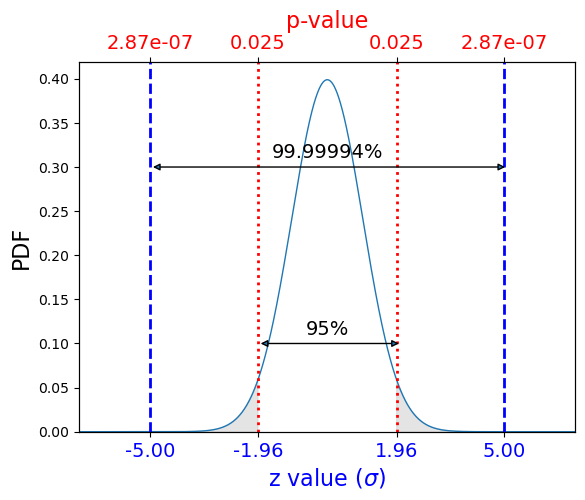
\includegraphics[scale=0.35]{StandardNormPvalZval.png}
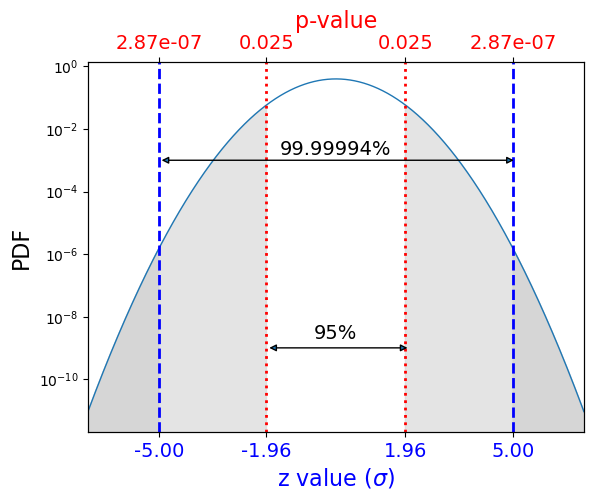
\includegraphics[scale=0.35]{StandardNormPvalZval-Log2sided.png}
\end{center}
\end{frame}





% P VALS FOR A FIT
\begin{frame}{P-values for a fit}
\footnotesize
Recall the Z-value and p-value are different ways of measuring the same thing:\\

$P(|Z| \leq \bbl{3}) = \rbl{99.73\%}$, \bbl{z-value is $3\sigma$}, \rbl{p-value is 0.0027}.\\[1ex]

A p-value of 0.0027 indicates that, given $H_0$, we would expect to observe this value for the data in $0.27\%$ of repeated experiments. A small p-value (large Z-value) is an indicator of rarity that is interpreted as 'highly significant'.\\[1ex]

When we think about probabilities in terms of fitting, our aim is to have the fit match the data as closely as possible, such that we can be confident in the parameter estimates.\\[1ex]

So, when we calculate the p-value for a fit, we do not find small p-values exciting! \magtn{A very small (or very large!) p-value for a fit means that we are very unlikely to have done a good job.}\\
\end{frame}



\begin{frame}{Degrees of Freedom}
\footnotesize
The number of degrees of freedom are central to many statistical tests.\\[1ex]


\magtn{Number of Degrees of Freedom}: \ghl{$\magtn{\nu} = N - \bbl{N_p} - \rbl{N_c}$}\\[3ex]

$N$: Number of measurements, aka sample size.\\[1ex]
\bbl{$N_p$: Number of parameters.}\\[1ex]
\rbl{$N_c$: Number of constraints.}\\[1ex]



\magtn{Example 1:} I have a dataset of 10 measurements, with a mean of $1.63$. How many degrees of freedom are there?\\[2ex]



\magtn{Example 2:} In a Least Squares fit I am estimating the parameters $m$ and $c$ of a straight line. I have 20 data points. How many degrees of freedom are there?\\[2ex]

%There are nine degrees of freedom, because I have nine values that are free, and the last one is constrained to the exact value needed to ensure the mean of all ten values is 1.63.\\[1ex]

%\magtn{Example 2:} If I have a dataset of 100 measurements, and I am estimating the variance, I have 99 degrees of freedom. This is because the variance estimate will require a sample mean, which constrains the dataset and therefore uses one degree of freedom.\\[1ex]

\end{frame}



\begin{frame}{Case Studies}
\footnotesize

\bbl{Normal} Tests ( Z-test, T-test, F-test):
\begin{enumerate}
\item Is the mean \bbl{height} of DAT students equal to the mean UK height?
\item Is the mean height of Mechanics students equal to that of DAT students?
%\item Do my two groups have the same variance?
\end{enumerate}
\vspace{0.5cm}

\magtn{Model} Tests ($\chi^2$, LLR, AIC, BIC):
\begin{enumerate}
%\item I have two datasets. Do they come from the same distribution?
\item My friend suggested a more complicated model might better fit my data. How do I prove him wrong?
\item What if he suggests a completely different model?
\end{enumerate}

\end{frame} 

%\begin{frame}{Constraints and Bounds}
%\footnotesize
%
%Bounds on a parameter are simple: we specify a range in which the parameter value must lie. \\[1ex]
%
%Constraints can be more complex, for example the sum or mean of the difference between the parameter value and x must be within some range.\\[1ex]
%
%Constraints can be powerful and are often needed in python optimisation algorithms.\\[1ex]
%
%There is a nice non-physics example of applying constraints (using the constraint that the angles of a triangle must sum to $180^{\circ}$) on pages 61-62 of the notes previously used for this module.
%\end{frame} 



\section*{Normal Tests}



% Z TEST
\begin{frame}{The Z Test}
\footnotesize
\bbl{Example usage}: test if the sample mean $\overline{x}$ equals a hypothesised mean $\mu_{_0}$.\\

\rbl{Restrictions}: Data are $X\sim Norm(\mu,\sigma)$, True Variance $\sigma^2$ is known. \\

\begin{center}
\bhl{$z= \dfrac{ \overline{x}-\mu_{_0} }{\sigma/\sqrt{N}}$}\\
\end{center}
The denominator $\sigma/\sqrt{N}$ is the standard error on the mean, $\sigma_{\overline{x}}$. \\

Reminder: \; \yhl{$V[\overline{x}] = V[X]/N  = \sigma^2/N \;\; \rightarrow \;\; \sigma_{\overline{x}} = \sigma /\sqrt{ N}$}. \\[1ex]

The test statistic z is standard normal, so we use \grhl{\texttt{from scipy.stats import norm}} for probabilities.
%\notsotiny
%\magtn{*I can't think of a feasible real-life situation where I would know the true variance but not the true mean, can you?}

\end{frame} 





% Z TEST EXAMPLE
\begin{frame}{Example of the Z Test}
\footnotesize
\bbl{Is the mean height of DAT students equal to the mean UK height?}\\

True Variance is known to be $\sigma^2=$ 50\,cm. The Null hypothesis is $H_0: \mu_{_0}=$ 170\,cm.\\
\begin{itemize}
\item $\alpha = 0.05$\hspace{1.7cm} \bbl{The significance level, chosen before looking at the data}.\\ 
\item $H_1: \mu \rbl{\neq}$ 170\,cm\hspace{0.75cm} \bbl{The Alternate Hypothesis.} \rbl{\ding{234} two-sided test.}\\
\item Statistics from data: $N=57$, $\overline{x}$=167\,cm.\\
\end{itemize}
\vspace{0.2cm}
%\rbl{We can see that 167 and 170 are not the same number. This test tells us how significantly they differ.}
\begin{center}
\bhl{$z = \dfrac{ \overline{x}-\mu_0 }{\sigma/\sqrt{N}} = \dfrac{167 - 170}{\sqrt{50/57}}  = -3.203$}\\[1ex]
\end{center}
The p-value is \grhl{\rbl{2} \texttt{* norm.sf(3.203)= 0.00136}}\;\ding{234}\;we reject $H_0$, because p$<\alpha$. \\[1ex]


\magtn{Note that} \grhl{\texttt{ norm.sf(|z|) = 1 - norm.cdf(|z|) = norm.cdf(-1*|z|)} }\\

\end{frame} 






% T TEST
\begin{frame}{The (\magtn{Student's})\magtn{*} T Test}
\footnotesize
\bbl{Example usage}: test if the sample mean $\overline{x}$ equals a hypothesised mean $\mu_{_0}$.\\

\rbl{Restrictions}: Data are approximately $X\sim Norm(\mu,\sigma)$. 
\begin{center}
\bhl{$T = \dfrac{ \overline{x}-\mu_0 }{\magtn{\sigma_{s}}/\sqrt{N}}$}\\
\end{center}

The \magtn{sample variance} used in the $T$ Test is an unbiased estimator for the true variance: 
$\magtn{
\sigma^2_{s}
} 
=  \dfrac{1}{N-1} \sum\limits_i^N (x_i - \overline{x} )^2$.\\[1ex]

T has its own PDF, so we use \grhl{\texttt{from scipy.stats import t}} for probabilities.\\

\scriptsize
\magtn{*Student} was the pen name of William Gosset. \href{https://en.wikipedia.org/wiki/William_Sealy_Gosset}{[wikipedia]}: "Gosset was a friend of both Pearson ($\chi^2$) and Fisher ($I_{\theta}$), a noteworthy achievement, for each had a massive ego and a loathing for the other." 
 
\end{frame} 





% T TEST EXAMPLE
\begin{frame}{Example of the T Test}
\footnotesize
\bbl{Same question: Is the mean height of DAT students equal to the mean UK height?}\\

As for the Z Test, $H_0: \mu_{_0}=$ 170\,cm, $\alpha = 0.05$, $H_1: \mu \rbl{\neq}$ 170\,cm\; \rbl{\ding{234} two-sided test.}\\
\begin{itemize}
\item Statistics from data: $N=57$, $\overline{x}$=167\,cm, \magtn{$\sigma_s=$10\,cm.}\\
\end{itemize}
\vspace{0.2cm}
\begin{center}
\bhl{$T= \dfrac{ \overline{x}-\mu_0 }{\sigma_s/\sqrt{N}} = \dfrac{167 - 170}{10/\sqrt{57}}  = -2.265$}\\[1ex]
\end{center}
The p-value is \grhl{\rbl{2} \texttt{* t.sf(2.265,\gbl{df=57-1})= 0.02740}}\; \ding{234}\; we reject $H_0$, as p$<\alpha$. \\[1ex]

\gbl{df = 57-1 is the Number of Degrees of Freedom, $\nu = N - N_p - N_c$.}\\

\magtn{Note that} \grhl{\texttt{ t.sf(|T|,df) = 1 - t.cdf(|T|,df) = t.cdf(-1*|T|,df)} }\\
\end{frame} 

\begin{frame}{Compare Z and T Tests}
\footnotesize
Z test found p-value \grhl{\texttt{2*norm.sf(3.203)= 0.00136}} using true $\sigma =$7\, cm.\\[1ex]

T test found p-value \grhl{\texttt{2*t.sf(2.265, df=57-1)= 0.02740}} using sample $\sigma_s =$10\, cm.\\[1ex]

\begin{multicols}{2}

Two things are happening here: the $\sigma$ are different, and the T distribution is not quite normal, it has fatter tails.\\[2ex]

Note that using $\sigma_s$ for the Z Test, the p-value \grhl{\texttt{norm.sf(2.265)}=0.0235 } \magtn{is smaller than for the T test}. \\[2ex]

\begin{center}
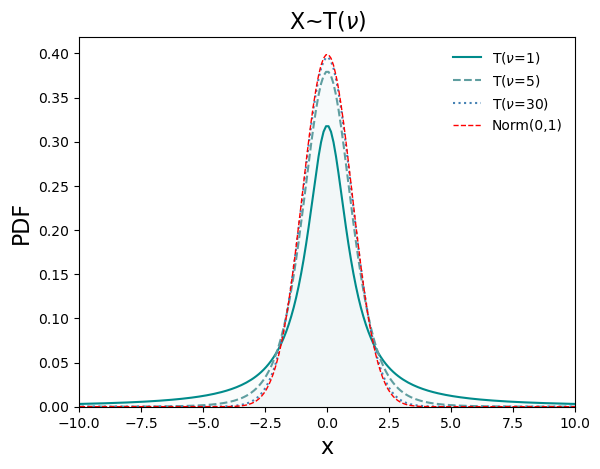
\includegraphics[scale=0.35]{StudentsT.png}
\end{center}

\end{multicols}
\end{frame} 




% TWO SAMPLE T TEST
% Z TEST
\begin{frame}{Two Sample T Test}
\footnotesize
\bbl{Example usage}: test if two samples have the same mean.\\

\rbl{Restrictions}: Data are $X\sim Norm(\mu,\sigma)$. Roughly equal variances ($0.5 < \dfrac{\sigma_x}{\sigma_y}< 2$). \\

\begin{center}
\bhl{$t = \dfrac{ \overline{x}-\overline{y} }{ \sigma_{p} }$}\\
\end{center}

The \magtn{ Pooled Variance}: $\magtn{\sigma^2_{p}} =  \dfrac{ 
\nu_x \sigma^2_{sx} 
+ \nu_y \sigma^2_{sy} 
}{\nu_x + \nu_y} 
$\\[1ex]

Here $\nu_x$ is the number of degrees of freedom for sample X ($\nu=N-1$), and $\sigma^2_{sx}$ is the variance of sample X.\\

%Otherwise "Welch's T Test": $\sigma^2_p =  \dfrac{\sigma^2_{sx} }{n } + \dfrac{\sigma^2_{sy} }{m}$


\end{frame} 


\begin{frame}{Example of the Two Sample T Test}
\footnotesize
\bbl{Are the mean heights of DAT students and Mechanics student equal?}\\[1ex]

The Null hypothesis is $H_0$: they are equal. We keep $\alpha = 0.05$.\\
The Alternate hypothesis is $H_1$: DAT are taller \magtn{\ding{234} one-sided test}.\\
\scriptsize
\begin{itemize}
\item DAT heights: $N=57$, $\overline{x}$=167\,cm. $\sigma_x=$10\,cm.\\
\item Mechanics heights: $N=53$, $\overline{x}$=165\,cm. $\sigma_x=$11\,cm.\\
\item $\sigma^2_{p} =  \dfrac{ \nu_x \sigma^2_{sx} + \nu_y \sigma^2_{sy} }{\nu_x + \nu_y} =
 \dfrac{ (57-1) 10^2 + (53-1) 11^2 }{(57-1)+ (53-1)} = 110$
\end{itemize}
\vspace{0.2cm}
\footnotesize
\begin{center}
\bhl{$t = \dfrac{ \overline{x}-\overline{y} }{ \sigma_{p} }
= (167 -165) / \sqrt{110} = 0.191
$}\\
\end{center}

The p-value is \grhl{\texttt{t.sf(0.191,\gbl{df=108})= 0.424}}\; \ding{234}\; we do not reject $H_0$, because p$>\alpha$. \\[1ex]

\scriptsize
We could perhaps have guessed this. T is roughly normal, and for $p<0.05$ we would need the means to be about 1.6 sigmas away from one another.
\end{frame} 






% F TEST
\begin{frame}{The $F$ Test (One-way ANOVA)}
\footnotesize
Another way to compare groups is via ANalysis Of VAriance. The F test is the ratio:\\

$F = 
\bhl{Variance\; between\; groups}
\bigg/
\ghl{Variance\; within\; groups}
$
\scriptsize
\begin{itemize}
\item $Z$ is the number of groups $j$, and $N$ is the number in each group $i$.
\item Mean of group $j$: $\overline{x}_j  = \frac{1}{N} \sum\limits_i^N  x_i$.
\item Variance of group $j$: $\sigma^2_{sj} = \frac{1}{N-1}  \sum\limits_i^N  (x_{ij} - \overline{x}_j)^2$.
\item Mean across all groups: $\overline{x} = \frac{1}{Z} \sum\limits_j^Z  \overline{x}_j$.
\end{itemize}
\footnotesize

$F =  $\bhl{$
\frac{1}{Z-1} \sum\limits_j^Z N_j (\overline{x}_j - \overline{x})^2
$}
$\bigg/$
\ghl{$\frac{1}{Z} \sum\limits_j^Z \sigma^2_{sj}$}\\[1ex]

F has its own PDF, so we use \grhl{\texttt{from scipy.stats import f}} for probabilities.\\
\end{frame} 


\begin{frame}{Example of the F Test}
\footnotesize
\bbl{Are the mean heights of DAT students and Mechanics student equal?}\\
%The Null hypothesis is $H_0$: they are equal. We keep $\alpha = 0.05$.\\
%The Alternate hypothesis is $H_1$: DAT are taller.\\
\scriptsize
\begin{itemize}
\item DAT heights: $N=57$, $\overline{x}$=167\,cm. $\sigma_x=$10\,cm.\\
\item Mechanics heights: $N=53$, $\overline{x}$=165\,cm. $\sigma_x=$11\,cm.\\
%\item $Z=2$ groups. $\overline{x} = \frac{1}{2}(167+165)= 166$ 
\item Variance between:  $\frac{1}{Z-1} \sum\limits_j^Z N_j (\overline{x}_j - \overline{x})^2
= \frac{1}{2-1} \left( 57(167-166)^2 + 53(165-166)^2 \right)= 110$
\item Variance within: $\frac{1}{Z} \sum\limits_j^Z \sigma^2_{sj}
= \frac{1}{2} (10^2 + 11^2) = 110.5$
\end{itemize}
\vspace{0.2cm}

\footnotesize
\begin{center}
\bhl{$F = \dfrac{ 110}{110.5} =0.995$}\\
\end{center}

Degrees of freedom: Variance between has $Z-1=1$, Variance within has $\sum_j N_j - Z =108$.\\

The p-value is \grhl{\texttt{f.sf(0.995,1,108)= 0.321}}\; \ding{234}\; we do not reject $H_0$, because p$>\alpha$. \\[1ex]

\end{frame} 


% CHI SQUARED
\section*{$\chi^2$}

\begin{frame}{Chi Squared and the Standard Normal RV}
\footnotesize
We have seen that $\chi^2$ is the statistic (the Loss Function) we minimise when using the Least Squares method to estimate parameters and their uncertainties. \\[1ex]

\begin{center}
\bhl{$\chi^2 = \sum\limits_i^N \dfrac{(y_i -\mu)^2 }{\sigma^2_i}$}\\[1ex]
\end{center}

It may have caught your eye that $\chi^2$ is the same form as the Standard Normal RV:\\[1ex]

\begin{center}
\ghl{ $Z = \dfrac{(x-\mu)}{\sigma}$}\\[1ex]
\end{center}

For a single measurement (a single \magtn{Degree of Freedom}), $\chi^2 = Z^2$. 
\end{frame}

\begin{frame}{Standard Normal Distribution}
\footnotesize
The Standard Normal distribution is familiar and welcoming.
%PDF: $f_Z(z) = \frac{1}{\sigma \sqrt{2\pi}} e^{-\frac{1}{2} z^2}$ and CDF: $F_Z(z) = \frac{1}{\sqrt{2\pi}}\int\limits_{-\infty}^{z} e^{-\frac{1}{2} z^2} dz$\\[1ex]
\begin{center}
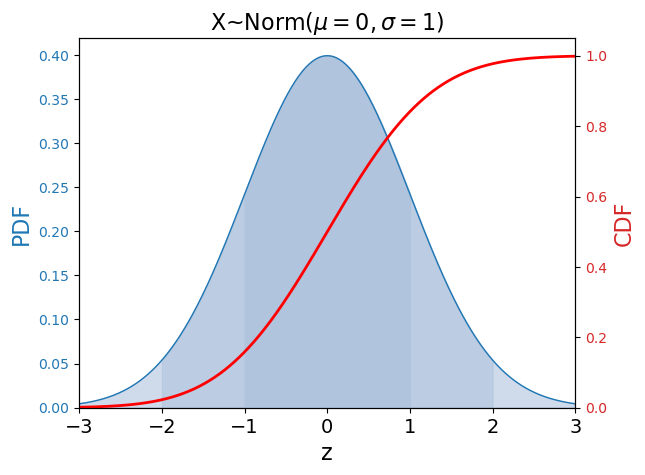
\includegraphics[scale=0.45]{StandardNorm.png}
\end{center}

\end{frame}


\begin{frame}{Chi Squared Distribution: 1 degree of freedom}
\footnotesize
The $\chi^2$ distribution looks weird, but makes sense.

\begin{center}
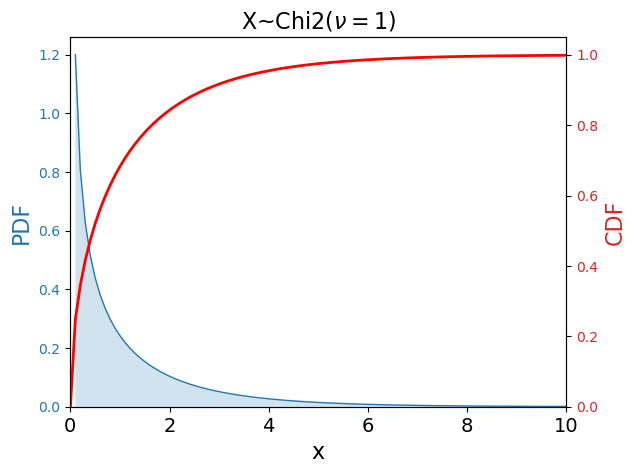
\includegraphics[scale=0.45]{Chi2-StandardNormLongTail.png}
\end{center}

\end{frame}


\begin{frame}{Chi Squared Distribution: 1 degree of freedom}
\footnotesize 
\begin{multicols}{2}

The x-axis is the size of the $\chi^2$  for our single measurement. \\

$x =\chi^2(\nu=1)=z^2 = \dfrac{(y_i-\mu)^2}{\sigma^2}$\\

The \rbl{CDF y-axis} is the probability of measuring a residual smaller or equal to that value.\\

$P(\chi^2 \leq x ) = F_x = \int\limits_{0}^x f_X dx$:\; \rbl{CDF}\\[1ex]


%PDF: $f_X(x;1) = \dfrac{1}{\pi \sqrt{2} } x^{-1/2}\, e^{-x/2}\;\;\; 0\leq x < \infty$. \\[1ex]

\begin{center}
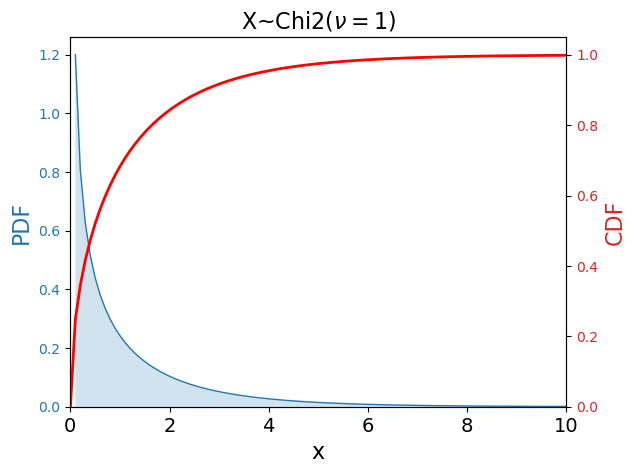
\includegraphics[scale=0.35]{Chi2-StandardNormLongTail.png}
\end{center}

\end{multicols}



The tail of the $Chi2(\nu)$ PDF goes to $\infty$ (I have truncated).
\end{frame}








%\begin{frame}{Chi Squared PDF}
%\footnotesize
%\begin{center}
%\bhl{$f_X(x;\nu) = \dfrac{2^{-\nu/2}}{\Gamma(\nu/2)  } x^{(\nu/2) - 1}\, e^{-x/2}\;\;\;for \;\;\; 0\leq x < \infty$} \\[1ex]
%\end{center}
%
%The  $\chi^2$ distributions are \gbl{sampling distributions}. Rather than describing the probabilities associated with waiting times, or heights, or some other real-world data, they describe the \gbl{probabilities of deviations from expectation}.\\[1ex]
%
%The parameter \magtn{$\nu$} is the \magtn{Number of Degrees of Freedom}: \ghl{$\magtn{\nu} = N - \bbl{N_p} - \rbl{N_c}$}\\[1ex]
%$N$: Number of measurements.\\[1ex]
%\bbl{$N_p$: Number of parameters.}\\[1ex]
%\rbl{$N_c$: Number of constraints.}\\[1ex]
%
%\end{frame}








\begin{frame}{Chi Squared PDF: a quick look}
\footnotesize
\begin{center}
\bhl{$f_X(x;\nu) = \dfrac{2^{-\nu/2} }{\Gamma(\nu/2) } x^{(\nu/2) - 1}\, e^{-x/2}\;\;\;for \;\;\; 0\leq x < \infty$} \\[1ex]
\end{center}

Number of Degrees of Freedom: $\magtn{\nu} = N - N_p - N_c$\\[1ex]

The \bbl{Expected Value} of $X \sim Chi2(\nu)$  is $E[X]=\nu$, \bbl{Variance} is $V[X] = 2\nu$.\\[1ex]

The $\Gamma(\nu/2)$ in the denominator is the \gbl{Gamma Function}: \ghl{$\Gamma(s) = \int\limits_0^{\infty} x^{s-1} e^{-x} dx$}. \\[2ex]

\scriptsize
The nice properties of this function include \magtn{$\Gamma(1/2)  = \sqrt{\pi}$},  \bbl{$\Gamma(n ) = (n-1)!$ where $n$ is a positive integer}, and \gbl{$\Gamma(s+1)  = s\Gamma(s)$}.\\[1ex]
$\nu=1\; \rightarrow \;  \Gamma(1/2) =\magtn{ \sqrt{\pi} }$\\[1ex]
$\nu=2\; \rightarrow \;  \Gamma(2/2) = \bbl{0! = 1}$\\[1ex]
$\nu=3\; \rightarrow \;  \Gamma(3/2) = \gbl{\Gamma(1/2 + 1)  =\frac{1}{2}} \magtn{\sqrt{\pi}}$\\[1ex]
%$\nu=4\; \rightarrow \;  \Gamma(4/2) = \bbl{1! = 1}$\\[1ex]
%$\nu=5\; \rightarrow \;  \Gamma(5/2) = \gbl{\Gamma(3/2 + 1)  =3\sqrt{\pi}/4}$\\[1ex]
and so on.\\

\footnotesize

\end{frame}







\begin{frame}{Chi Squared Distribution}
\footnotesize
When we increase the degrees of freedom, the probability distribution for $\chi^2$ completely changes, because \magtn{$\chi^2$ is the sum} of the squared residuals.

\begin{center}
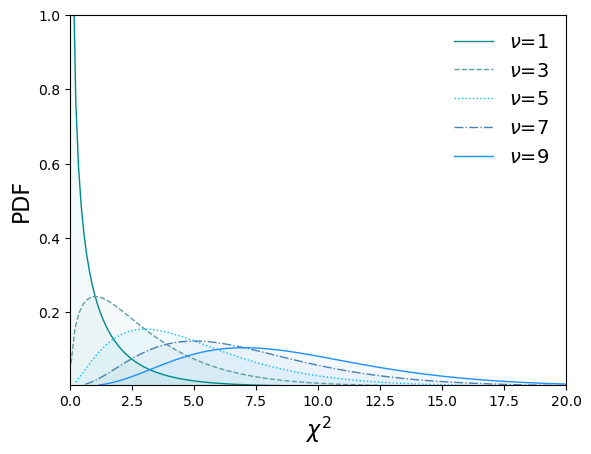
\includegraphics[scale=0.45]{Chi2-nus-liny-smallsteps.png}

\end{center}

\end{frame}


\begin{frame}{Reduced Chi Squared ($\chi^2/\nu$) Distribution}
\footnotesize
%The reduced $\chi^2$ is divided by the number of degrees of freedom $\nu$. 
Dividing the $\chi^2$ by its Expected Value, $E[\chi^2]=\nu$, standardises it. As we increase $\nu$, the $\chi^2/\nu$ distribution approaches Norm($\mu=1, \sigma = \sqrt{ 2/\nu}$).

\begin{center}
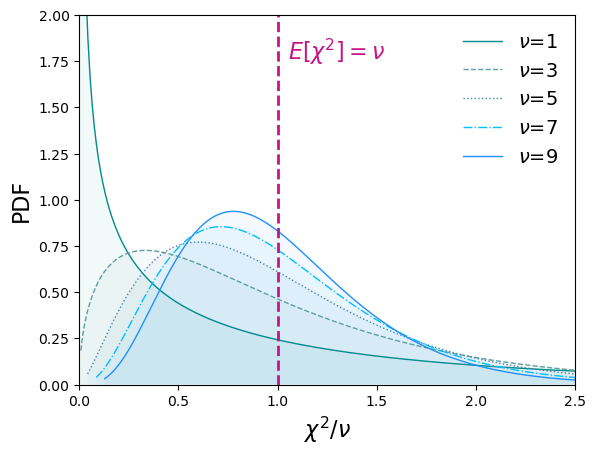
\includegraphics[scale=0.35]{Chi2-nus-liny-smallsteps-pdf-reduced.png}
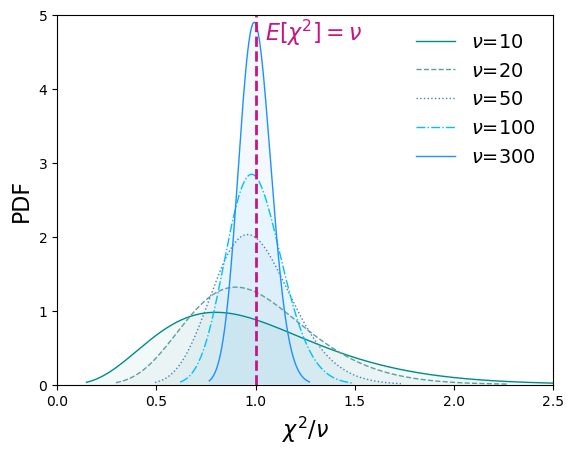
\includegraphics[scale=0.35]{Chi2-nus-liny-bigsteps-pdf-reduced.png}
\end{center}

\end{frame}


\begin{frame}{Reduced Chi Squared ($\chi^2/\nu$) Probability}
\footnotesize
The reduced $\chi^2/\nu$ p-value (1-CDF) allow us to view our fit as a hypothesis, and reject it if it falls below some predefined \rbl{significance level $\alpha$}.\\[1ex] %Be careful when using $\chi^2/\nu$ for this.

\begin{center}
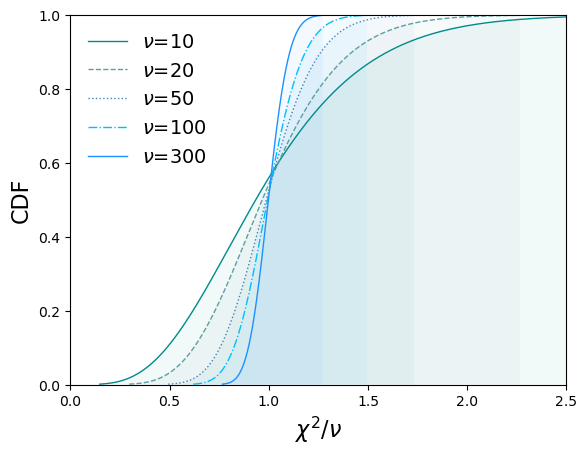
\includegraphics[scale=0.33]{Chi2-nus-liny-bigsteps-cdf-reduced.png}
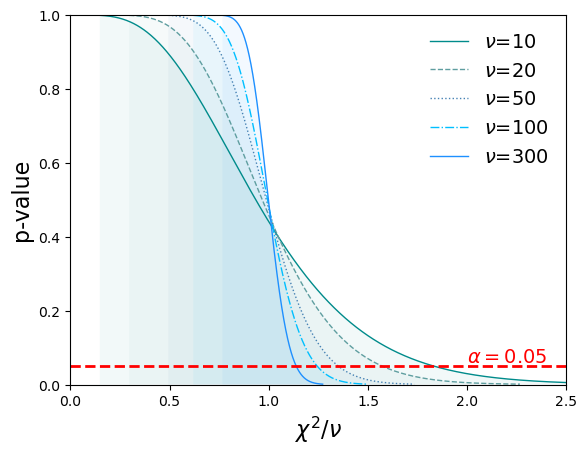
\includegraphics[scale=0.33]{Chi2-nus-liny-bigsteps-pvalue-reduced.png}
\end{center}

\end{frame}




\begin{frame}{Reduced Chi Squared ($\chi^2/\nu$) Probabilities}
\footnotesize

\bbl{The $\chi^2/\nu$ should be close to 1. If it is much higher, this indicates a poor fit. If it is much lower, this indicates the uncertainty estimates are too large (overfitting).}\\[1ex]

\magtn{You should state your fit results as eg $\chi^2/\nu = 15/10$ and NOT as eg $\chi^2/\nu = 1.5$}. \\[1ex]

%\notsotiny
\begin{multicols}{2}
$P(\chi^2 \geq 15 | \nu=10 ):$\\[1ex]
\grhl{\texttt{chi2.sf(15,10)=0.132} }\\[1ex]
\gbl{okay} \\[2ex]

$P(\chi^2 \geq 150 | \nu=100 ):$\\[1ex]
\grhl{\texttt{chi2.sf(15,10)=0.001}}\\[1ex]
 \rbl{excluded!}\\[1ex]

%$P(\chi^2 \geq 1 | \nu=10 ) =$ \; \texttt{ 1-( chi2.cdf(1,10)  ) = 0.9998} \\[1ex]
%$P(\chi^2 \geq 17 | \nu=12 ) =$ \; \texttt{ 1-( chi2.cdf(17,12)  ) = 0.150} \\[1ex]
%%
%%\rbl{p-value}: \texttt{ 1- ( norm.cdf(1) - norm.cdf(-1) ) = 0.3173}\\[1ex]
%%\texttt{ chi2.cdf(1,1) = 0.683} \rbl{p-value}: \texttt{ 1- ( chi2.cdf(1,1)  ) = 0.3173}\\[1ex]
%%\texttt{ chi2.cdf(1,2) = 0.393}
%%\texttt{ chi2.cdf(1,10) = 0.00017}
%%$\nu=1$: \texttt{ chi2.cdf(1,1) = 0.683} :A $\chi^2 \geq 1$ ($|Z|>1\sigma$) will be observed in p=$31.7\%$ of cases \\[1ex]
%%%$\nu=1$: \texttt{ chi2.cdf(4,1) = 0.9545} :A $\chi^2 \geq 4$  ($|Z|>2\sigma$) will be observed in p=$4.55\%$ of cases \\[1ex]
%%$\nu=10$: \texttt{ chi2.cdf(7.4,10) = 0.313} :A $\chi^2 \geq 7.4$  will be observed in p=$68.7\%$ of cases \\[1ex]
%
%\rbl{Note:}\\[1ex]
%You should state your fit results as eg $\chi^2/\nu = 17/12$ and NOT as eg $\chi^2/\nu = 1.42$, because the latter could have any pair of values, for example $\chi^2/\nu = 170/120$:\\[1ex]
%
%$P(\chi^2 \geq 170 | \nu=120 ) =$ \; \texttt{ 1-( chi2.cdf(170,120)  ) = 0.0018} \\[1ex]
%
%With $\alpha=0.05$, this (p-value= 0.0018) fit would then be (incorrectly!) excluded as a valid description of  the data.

\begin{center}
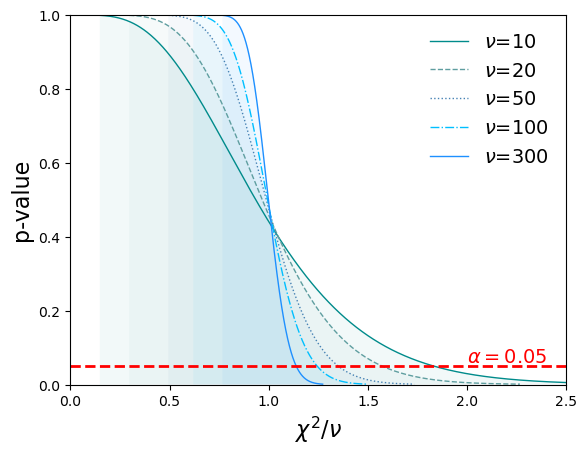
\includegraphics[scale=0.35]{Chi2-nus-liny-bigsteps-pvalue-reduced.png}
\end{center}


\end{multicols}
\footnotesize

\end{frame}


% GOODNESS OF FIT
\section*{Model Tests}

% LLR
\begin{frame}{Likelihood Ratio Test for Goodness of fit}
\footnotesize
The Log Likelihood Ratio Test is \yhl{$LLR =  - 2  \ln  \dfrac{ \mathcal{L}_A }{ \mathcal{L}_B } = - 2  (\ln \mathcal{L}_A  - \ln \mathcal{L}_B )$}.\\[1ex]

To use this method, \bbl{$\mathcal{L}_A$ must be a simplified version of $\mathcal{L}_B$}. \\[1ex]%For example, $\mathcal{L}_A$ might cover a smaller region of parameter space, or have fewer parameters, but it must be possible to build $\mathcal{L}_B$ from $\mathcal{L}_A$.\\[1ex]


\magtn{Example 1}: $\mathcal{L} = \prod\limits_i^N f_{X} $, where $f_{X,A} =  ax^3$ and $f_{X,B} =  ax^3 / ( 1+ bx) $. Model A has $N_p=1$ parameters, Model B has $N_p=2$. \bbl{Model A is nested in Model B}, because if $b=0$, they are the same. \gbl{The difference in $\nu$ is $|\nu_A - \nu_B| = 1$}.\\

\magtn{Example 2}: $f_{X,A} =  ax^3,\;\;\;0.1<a<0.2$ and $f_{X,B} =  ax^3,\;\;\;0 <a<1$. \bbl{A has an additional constraint} with respect to model B. \gbl{$|\nu_A - \nu_B| = 1$} \\



We could then use \grhl{\texttt{pvalue=chi2.sf(LLR, df=1)}}: if  \texttt{pvalue} $< \alpha$, we reject the simpler model, A, in favour of its more complicated friend, B. But, there are other ways of doing this with LLR - more next week.\\

\end{frame} 









% GOODNESS OF FIT
\begin{frame}{Comparing Un-nested models: AIC and BIC}
\footnotesize
If we want to compare un-nested models, we can use the AIC or BIC statistics. \magtn{They both balance the simplicity of the model ($k$: number of model parameters) with the quality of fit to data}.\\[1ex]

The Akaike Information Criterion (AIC):
\begin{center}
\bhl{$\mathsf{AIC} =  2k - 2 \ln \mathcal{L}_{\hat{\theta}}$}\\
\end{center}
\vspace{0.3cm}

The Bayesian Information Criterion (BIC):
\begin{center}
\bhl{$\mathsf{BIC} =  k \ln N - 2 \ln \mathcal{L}_{\hat{\theta}}$}\\
\end{center}

\magtn{A smaller Information Criterion value is better}, eg $\mathsf{AIC}_{\alpha} < \mathsf{AIC}_{\beta}$ identifies the preferred model as $\alpha$.\\

% is argued to be appropriate for selecting the "true model" (i.e. the process that generated the data) from the set of candidate models. However, the true model will almost never be in the set of candidate models. \magtn{`All models are wrong.'} is an approximation to the Bayes Factor: 
\end{frame} 


\begin{frame}{Akaike Information Criteria Example}
\footnotesize

Last week we tossed a coin 50 times and it came up heads 27 times.\\[2ex]

\bbl{The Likelihood under Model $\alpha$ (p=0.5):} \\
 $\mathcal{L}_{\alpha} = \dfrac{50!}{27! 23!} 0.5^{27} 0.5^{23} = 0.09596$\\[2ex]

\footnotesize
\bbl{The Likelihood under Model $\beta$ (p=27/50):} \\
$\mathcal{L}_{\beta} = \dfrac{50!}{27! 23!} (27/50)^{27} (23/50)^{23} = 0.11263$\\[2ex]
\footnotesize

$\mathsf{AIC}_{\alpha} =  2k - 2 \ln \mathcal{L}_{\alpha} = 2 - 2 \ln (0.09596)  = 6.6876$\\[1ex]
$\mathsf{AIC}_{\beta} =  2k - 2 \ln \mathcal{L}_{\beta} = 2 - 2 \ln (0.11263)  = 6.3673$\;\;\;  \magtn{$\leftarrow$ smaller preferred} \\

\end{frame}


\begin{frame}{AIC probabilities }
\footnotesize

We identify the minimum: $\mathsf{m} = \mathsf{min}( \mathsf{AIC}_{\alpha}, \mathsf{AIC}_{\beta}) = \mathsf{min}( 6.6876, 6.3673) = 6.3673 $ \\[1ex]

The \magtn{Relative Likelihoods} for AIC are:\\[1ex]
$r_{\alpha} = \exp[\frac{1}{2}( m - \mathsf{AIC}_{\alpha})] = \exp[\frac{1}{2}( 6.3673 - 6.6876)] = 0.852$\\[1ex]
$r_{\beta} = \exp[\frac{1}{2}( m - \mathsf{AIC}_{\beta})] = \exp[\frac{1}{2}( 6.6876 - 6.6876)] = 1$\\[1ex]

The \magtn{Akaike Weights} are then: \\[1ex]
$p_{\alpha} = r_{\alpha}/(r_{\alpha} + r_{\beta}) = 0.852/1.852 = 0.460$\\[1ex]
$p_{\beta} = r_{\beta}/(r_{\alpha} + r_{\beta}) = 1/1.852 = 0.540$\\[1ex]

The weight $p_{\beta}$ is the probability that $p=27/50$ is the best of the two options, given the data. Generally, if the difference \magtn{$|\mathsf{AIC_{\alpha}} - \mathsf{AIC_{\beta}}| < 2 $} it is classified as \magtn{not worth more than a bare mention} - see \href{https://sites.stat.washington.edu/raftery/Research/PDF/kass1995.pdf}{  [Kass 1995]}.% and this \href{https://royalsocietypublishing.org/doi/10.1098/rspb.2023.1261}{nice RS paper}.
\end{frame} 



%\section*{Resampling}
%
%
%\begin{frame}{Resampling}
%\footnotesize
%Subsampling from a sample with replacement is called resampling.\\
%
%\end{frame} 
%
%
%\begin{frame}{Bootstrap}
%\footnotesize
%To bootstrap, you 
%
%
%\end{frame} 
%
%\begin{frame}{Jackknife}
%\footnotesize
%
%\end{frame} 




%$LR = 2  \ln \dfrac{ 0.11263}{0.095962 }  =0.32034$\\
%
%%The number of degrees of freedom is $\nu=1$ ($N=1, N_c=0, N_p=0$).\\
%\texttt{ chi2.cdf(0.32034,df=1) = 0.42860}: the LR test supports $H_0$ with $\sim 57\%$ confidence.
%
%\bbl{The Likelihood under the Null Hypothesis (p=0.5):} $\mathcal{L}_0 = \dfrac{50!}{27! 23!} 0.5^{27} 0.5^{23} = 0.095962$\\[1ex]
%
%\bbl{The Likelihood under the Alternate Hypothesis (p=27/50):} $\mathcal{L}_1 = \dfrac{50!}{27! 23!} (27/50)^{27} (23/50)^{23} = 0.11263$\\[1ex]
%
%$BIC_0 =  k\ln N - 2 \ln \mathcal{L}_0 = 0 - 2 \ln (0.09596) =  4.6876$\\
%$BIC_1 =  k\ln N - 2 \ln \mathcal{L}_1 = 0 - 2 \ln (0.11263) =  4.3673$\;\;\;  $\leftarrow$ smaller preferred \\
%



%These methods are reduced to being the same for this quite silly example.\\

\begin{frame}{Thanks For Your Time}
\center
\Huge
Fin.
\end{frame}

\end{document}



0027[1